\chapter{Photonenbahnen, Rindler-Raum und das Innere der Schwarzschild-Lösung}

Eine Newtonsche Punktmasse und ein Schwarzschild-Schwarzes-Loch gehen von derselben Idealisierung aus: Die gesamte gravitative Masse ist im Zentrum konzentriert. Dennoch bedeutet ihr jeweiliges Zentrum etwas grundlegend anderes. In der Newtonschen Mechanik verfehlt ein Teilchen das Zentrum schon bei einem noch so kleinen Drehimpuls. In einem Schwarzen Loch lässt sich die Singularität nach dem Überqueren des Horizonts nicht mehr verfehlen. Um diesen Unterschied zu verstehen, betrachten wir Kreisbahnen, die Photonensphäre und schließlich ein neues Koordinatensystem in Horizontnähe.

\section{Ein Zentrum, das sich nicht verfehlen lässt}

Reale Newtonsche Materie wird niemals zu einem mathematischen Punkt. Druck, Materialfestigkeit und andere Kräfte wirken der Kompression entgegen. Selbst wenn wir eine Punktmasse dennoch als Idealisierung verwenden, trifft ein fallendes Teilchen sie nur selten. Eine exakt radiale Bahn kann \(r=0\) erreichen, doch schon die kleinste transversale Geschwindigkeit verleiht dem Teilchen Drehimpuls. Die Zentrifugalbarriere lenkt es dann um das Zentrum herum.

In der allgemeinen Relativitätstheorie fällt die Antwort anders aus. Ein hinreichend kompakter Körper kann ein Schwarzes Loch bilden, und im Inneren des Schwarzen Lochs gibt es kein Newtonsches Ausweichen um das Zentrum. Der Grund liegt tiefer als in einer stärkeren Kraft: Innerhalb des Horizonts ist eine Abnahme von \(r\) eine Richtung in die Zukunft. Zu dieser Aussage gelangen wir schrittweise, statt sie einfach vorauszusetzen.

\begin{classroomqa}
\audiencequestion{Ist es bei der Newtonschen Schwierigkeit, das Zentrum zu treffen, lediglich eine Folge davon, dass beide Objekte als Punkte behandelt werden?}
\lecturerresponse{Die Punktidealisierung gehört zu diesem Vergleich, erklärt den Unterschied aber nicht vollständig. In der Newtonschen Mechanik kann eine Bahn bei jedem von null verschiedenen Drehimpuls um den Punkt herumführen. Im relativistischen Inneren liegt die Singularität in der Zukunft jeder einfallenden zeitartigen Bahn; eine Winkelbewegung kann kein Entkommen ermöglichen.
\lecturetimestamp{00:04:52--00:05:13}}
\end{classroomqa}

\section{Horizont und Singularität}

Wir setzen die Schwarzschild-Geometrie zunächst voraus:
\begin{equation}
d\tau^{2}
=
\left(1-\frac{2MG}{r}\right)dt^{2}
-
\frac{dr^{2}}{1-\frac{2MG}{r}}
-
r^{2}d\Omega^{2}.
\label{eq:l6-schwarzschild}
\end{equation}
Die Feldgleichungen, die diese Metrik festlegen, behandeln wir später. Zunächst wollen wir verstehen, was die Metrik aussagt.

Die Metrik der Einheitskugel lässt sich schreiben als
\begin{equation}
d\Omega^{2}
=d\vartheta^{2}+\cos^{2}\vartheta\,d\phi^{2}
\label{eq:l6-angular-metric}
\end{equation}
wobei \(\vartheta\) die vom Äquator aus gemessene Breite bezeichnet. Beim gebräuchlicheren Polarwinkel, der von der Achse aus gemessen wird, tritt an die Stelle des Kosinus ein Sinus. Aufgrund der Kugelsymmetrie lässt sich jede Bahn in eine feste Ebene legen, sodass in der folgenden Rechnung nur eine Winkelkoordinate vorkommt.

\begin{figure}[htbp]
\centering
\includegraphics[width=0.88\textwidth]{lecture_06_figure_01.png}
\caption{Die Schwarzschild-Metrik und die zylindrische Raumzeitdarstellung der Fläche \(r=2MG\). Die zentrale Linie ist \(r=0\); der rote Zylinder stellt den Horizont in Schwarzschild-Koordinaten dar.}
\lectureframe{00:09:45}
\end{figure}

Weit von der Quelle ist \(2MG/r\) klein, und
~\eqref{eq:l6-schwarzschild} nähert sich der Minkowski-Metrik in Kugelkoordinaten. Zwei Radien sind besonders wichtig:
\begin{equation}
r=2MG,
\qquad
r=0.
\end{equation}
Sie dürfen nicht verwechselt werden. Bei \(r=2MG\) verschwindet der Koeffizient von \(dt^{2}\), während der von \(dr^{2}\) divergiert. Das Schwarzschild-Koordinatensystem ist dort singulär geworden. Die Krümmung selbst bleibt an dieser Stelle endlich. Bei \(r=0\) dagegen divergieren Krümmungsinvarianten. Das Gezeitenfeld dehnt einen ausgedehnten Körper radial und staucht ihn transversal unbegrenzt. Das ist eine physikalische Singularität, kein Koordinatenfehler.

\subsection{Zwei Arten, einen Fall zu messen}

Für eine ruhende Uhr außerhalb des Horizonts gilt
\begin{equation}
d\tau
=
\sqrt{1-\frac{2MG}{r}}\,dt.
\label{eq:l6-static-clock}
\end{equation}
Bei großen \(r\) gilt \(d\tau\simeq dt\). In Horizontnähe vergeht die Eigenzeit einer Uhr, die bei festem \(r\) gehalten wird, gegenüber der weit entfernt gemessenen Schwarzschild-Zeit sehr langsam.

In denselben Koordinaten dauert der radiale Fall bis \(r=2MG\), gemessen durch \(t\), unendlich lange. Die Eigenzeit, die der Fallende selbst erlebt, ist endlich. Darin liegt kein Widerspruch. Eine mit dem Fallenden mitgeführte Uhr misst die Eigenzeit entlang seiner Weltlinie. Das kann eine mechanische Uhr sein, eine Lichtuhr mit Spiegeln an den Enden eines Meterstabs, ein Herzschlag oder die Abfolge physikalischer Prozesse im Gehirn. Nichts davon misst die Koordinatenzeit \(t\), wie sie in der Ferne definiert ist. Im Horizontdiagramm wird der Unterschied zwischen den beiden Uhren sichtbar.

\section{Kreisbewegung aus der Eigenzeit-Wirkung}

Bevor wir zum Fall zurückkehren, lösen wir ein anderes Problem: Unter welchen Bedingungen können ein massives Teilchen oder ein Photon das Schwarze Loch auf einer Kreisbahn umkreisen? Die Rechnung beginnt mit demselben Wirkungsprinzip wie bei jedem frei beweglichen relativistischen Teilchen:
\begin{equation}
S=-m\int d\tau.
\label{eq:l6-particle-action}
\end{equation}
Licht wird von der Erde abgelenkt, doch das irdische Gravitationsfeld ist bei Weitem nicht stark genug, um einen Lichtstrahl auf eine geschlossene Bahn zu zwingen. Der Schwarzschild-Radius der Erde beträgt nur ungefähr einen Zentimeter. Erst wenn man die gesamte Erde auf etwa diese Größenordnung, ungefähr die Größe einer kleinen Nuss, komprimierte, wäre die Frage nach dem starken Feld relevant.

Wir setzen \(c=1\), beschränken die Bewegung auf die Äquatorebene und definieren
\begin{equation}
F(r)=1-\frac{2MG}{r},
\qquad
G(r)=\frac{1}{F(r)}.
\label{eq:l6-fg}
\end{equation}
Verwenden wir die Koordinatenzeit \(t\) als Parameter, erhalten wir
\begin{equation}
d\tau
=dt\sqrt{F-G\dot r^{\,2}-r^{2}\dot\theta^{\,2}},
\end{equation}
und damit
\begin{equation}
\mathcal L
=
-m\sqrt{F-G\dot r^{\,2}-r^{2}\dot\theta^{\,2}}.
\label{eq:l6-lagrangian}
\end{equation}
Der Faktor \(m\) verleiht der Wirkung die üblichen Einheiten von Energie mal Zeit.

\begin{figure}[htbp]
\centering
\includegraphics[width=0.76\textwidth]{lecture_06_figure_02.png}
\caption{Die Wurzel-Lagrange-Funktion des Teilchens entsteht an der Tafel. Der vollständige Ausdruck steht in Gl. ~\eqref{eq:l6-lagrangian}.}
\lectureframe{00:31:53}
\end{figure}

Für jede verallgemeinerte Koordinate \(q\) gilt
\begin{equation}
p_q=\frac{\partial\mathcal L}{\partial\dot q}.
\end{equation}
Es ist zweckmäßig, \(\mathcal L\) für die Lagrange-Funktion und \(L\) für den Drehimpuls zu verwenden. Mit
\begin{equation}
\Delta=F-G\dot r^{\,2}-r^{2}\dot\theta^{\,2},
\end{equation}
lauten die beiden Impulse
\begin{align}
L=p_\theta
&=\frac{mr^{2}\dot\theta}{\sqrt{\Delta}},
\label{eq:l6-angular-momentum}\\
p_r
&=\frac{mG\dot r}{\sqrt{\Delta}}.
\label{eq:l6-radial-momentum}
\end{align}
Der Radialimpuls ist nicht erhalten, weil die Radialkoordinate in der Lagrange-Funktion vorkommt. Der Winkel \(\theta\) kommt darin nicht vor, also ist \(L\) erhalten.

Außerdem kommt \(t\) nicht explizit in \(\mathcal L\) vor. Daher ist der Hamiltonian erhalten:
\begin{align}
E=H
&=p_r\dot r+L\dot\theta-\mathcal L \\
&=\frac{mG\dot r^{\,2}}{\sqrt{\Delta}}
  +\frac{mr^{2}\dot\theta^{\,2}}{\sqrt{\Delta}}
  +m\sqrt{\Delta} \\
&=\frac{mF}{\sqrt{\Delta}}.
\label{eq:l6-energy-general}
\end{align}
Das ist ein typischer Ablauf in der Mechanik. Ein Prinzip liefert die Wirkung; aus einer Rechnung ergeben sich die Impulse; Symmetrien führen dann zurück zu den Erhaltungssätzen für Energie und Drehimpuls. Man könnte sofort sämtliche Euler--Lagrange-Gleichungen lösen, aber die Konstanten, die aus der Rotations- und Zeittranslationssymmetrie folgen, ersparen einen Großteil dieser Arbeit.

\subsection{Die Energie der Kreisbahn}

Für eine Kreisbahn gilt
\begin{equation}
\dot r=0.
\end{equation}
Wir führen den Drehimpuls pro Masseneinheit ein:
\begin{equation}
\lambda=\frac{L}{m}.
\end{equation}
Aus den Gleichungen ~\eqref{eq:l6-angular-momentum} und
\eqref{eq:l6-energy-general} folgt
\begin{align}
\lambda
&=\frac{r^{2}\dot\theta}
{\sqrt{F-r^{2}\dot\theta^{\,2}}},
\label{eq:l6-lambda-circular}\\
E
&=\frac{mF}{\sqrt{F-r^{2}\dot\theta^{\,2}}}.
\label{eq:l6-energy-circular-first}
\end{align}

\begin{figure}[htbp]
\centering
\includegraphics[width=0.82\textwidth]{lecture_06_figure_04.png}
\caption{Reduzierter Drehimpuls und Energie für eine Kreisbewegung in der Schwarzschild-Geometrie. Zuerst wird die Drehimpulsgleichung verwendet, um \(\dot\theta\) aus der Energie zu eliminieren.}
\lectureframe{00:39:14}
\end{figure}

Quadrieren wir Gl. ~\eqref{eq:l6-lambda-circular} und lösen nach der Winkelgeschwindigkeit auf, ergibt sich
\begin{equation}
\dot\theta^{\,2}
=
\frac{\lambda^{2}F}
{r^{2}\left(r^{2}+\lambda^{2}\right)}.
\label{eq:l6-angular-speed}
\end{equation}
Setzen wir dies in Gl. ~\eqref{eq:l6-energy-circular-first} ein, bleibt eine Energie, die nur vom angenommenen Radius und vom festen Drehimpuls abhängt:
\begin{equation}
E(r,\lambda)
=m\sqrt{F(r)}\,\frac{\sqrt{r^{2}+\lambda^{2}}}{r}.
\label{eq:l6-circular-energy}
\end{equation}

Die Vorlesung macht einen kurzen Vergleich mit der Newtonschen Mechanik. Bei einer gewöhnlichen Kreisbahn nehmen sowohl die Winkelgeschwindigkeit als auch die Tangentialgeschwindigkeit mit wachsendem Radius ab, der Drehimpuls enthält jedoch einen Radiusfaktor. Deshalb lässt sich das Verhalten von \(L\) nicht allein aus der Winkelgeschwindigkeit ableiten. In der relativistischen Formel sind diese Faktoren ausdrücklich sichtbar.

\section{Die Kreisbahn des Lichts}

Ein Photon besitzt Energie und Impuls, obwohl seine Ruhemasse verschwindet. Der masselose Grenzfall von Gl. ~\eqref{eq:l6-circular-energy} muss daher sorgfältig gebildet werden. Würde \(m\) bei festem \(\lambda\) gegen null gehen, dann würde auch \(L=m\lambda\) verschwinden. Stattdessen betrachten wir den Grenzfall
\begin{equation}
m\longrightarrow0,
\qquad
\lambda\longrightarrow\infty,
\qquad
L=m\lambda\ \text{fixed}.
\label{eq:l6-massless-limit}
\end{equation}
Dann dominiert der Term \(\lambda^{2}\), und die Photonenergie lautet
\begin{equation}
E_\gamma(r;L)
=L\,\frac{\sqrt{1-\frac{2MG}{r}}}{r}.
\label{eq:l6-photon-energy}
\end{equation}
Der Faktor \(L\) multipliziert die gesamte Radialfunktion. Er beeinflusst die Energieskala, nicht aber den Radius einer Kreisbahn.

\begin{figure}[htbp]
\centering
\includegraphics[width=0.88\textwidth]{lecture_06_figure_05.png}
\caption{Der Radialfaktor in der Photonenergie. Er verschwindet am Horizont, fällt bei großen Radien gegen null und besitzt dazwischen genau ein Maximum.}
\lectureframe{00:50:50}
\end{figure}

Bei festem \(L\) erfordert das radiale Gleichgewicht einen stationären Punkt:
\begin{equation}
\frac{d}{dr}
\left[
\frac{\sqrt{1-\frac{2MG}{r}}}{r}
\right]=0.
\end{equation}
Durch Differenzieren erhalten wir
\begin{equation}
-\frac{\sqrt{1-\frac{2MG}{r}}}{r^{2}}
+
\frac{MG}
{r^{3}\sqrt{1-\frac{2MG}{r}}}
=0,
\end{equation}
und somit
\begin{equation}
r=3MG.
\label{eq:l6-photon-sphere}
\end{equation}
Dieser Radius beträgt das Eineinhalbfache des Schwarzschild-Radius. Üblicherweise nennt man ihn Photonensphäre.

Der stationäre Punkt ist ein Maximum, daher ist die Kreisbahn des Photons instabil. Ein Photon, das sich genau bei \(3MG\) befindet, bleibt dort. Eine noch so kleine radiale Auslenkung führt dazu, dass es sich schließlich vom Maximum entfernt. Knapp außerhalb der Photonensphäre kann ein Lichtstrahl einen sehr großen Winkel überstreichen und womöglich viele Male um das Schwarze Loch laufen, bevor er entkommt. Knapp innerhalb davon kann ein nahezu tangentialer Strahl einige Umläufe vollziehen und dann durch den Horizont fallen.

\begin{figure}[htbp]
\centering
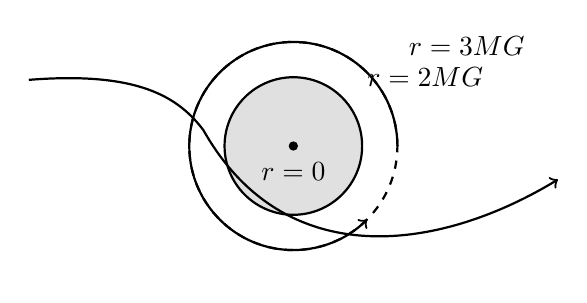
\begin{tikzpicture}[scale=1.12]
\fill[black!12] (0,0) circle (0.78);
\draw[thick] (0,0) circle (0.78);
\draw[dashed,thick] (0,0) circle (1.18);
\fill (0,0) circle (1.5pt);
\draw[->,thick] (1.18,0) arc (0:315:1.18);
\draw[->,thick] (-3.0,0.75)
  .. controls (-1.75,0.85) and (-1.30,0.55) .. (-1.02,0.18)
  .. controls (-0.10,-1.45) and (1.65,-1.20) .. (3.0,-0.38);
\node[right] at (0.73,0.78) {\(r=2MG\)};
\node[right] at (1.20,1.13) {\(r=3MG\)};
\node[below] at (0,-0.08) {\(r=0\)};
\end{tikzpicture}
\caption{Der Horizont, die Photonensphäre und ein stark abgelenkter Lichtstrahl. Strahlen, die der instabilen Kreisbahn beliebig nahe kommen, können vor dem Entkommen oder dem Hineinfallen beliebig große Ablenkungen ansammeln.}
\end{figure}

\begin{classroomqa}
\audiencequestion{Warum hält man den Drehimpuls fest, und wie hängt er mit der Frequenz eines Photons und seiner einfallenden Bahn zusammen?}
\lecturerresponse{Jeder Strahl besitzt einen erhaltenen Drehimpuls um das Schwarze Loch. Seine Frequenz legt den Betrag seines linearen Impulses fest, während sein Abstand vom Zentrum zur Bestimmung von \(L\) beiträgt. Abseits einer Kreisbahn können Radius und Drehimpuls unabhängig voneinander gewählt werden. Die Forderung nach einer Kreisbahn des Photons verknüpft die Bewegung mit dem eindeutigen Radius \(3MG\), und die Faktorisierung in Gl. ~\eqref{eq:l6-photon-energy} zeigt, dass dieser Radius unabhängig vom Betrag von \(L\) ist.
\lecturetimestamp{00:54:43--00:57:02}}
\end{classroomqa}

\begin{classroomqa}
\audiencequestion{Warum bestimmt das Maximum der Energie den Radius einer Bahn?}
\lecturerresponse{Nachdem wir die Winkelbewegung bei festem \(L\) eliminiert haben, spielt die verbleibende Funktion die Rolle einer effektiven radialen Energie. Ein stationärer Punkt ergibt radiales Gleichgewicht. Ein Minimum wäre stabil; hier liegt jedoch ein Maximum vor, das eine instabile Kreisbahn ergibt. Es ist kein Widerspruch, sie zugleich als Gleichgewicht und als instabil zu bezeichnen.
\lecturetimestamp{00:57:51--00:58:54}}
\end{classroomqa}

Ein massives Teilchen kann zeitartige Kreisbahnen außerhalb von \(3MG\) haben, doch die nächstgelegenen zur Photonensphäre sind instabil. Ein masseloses Teilchen besitzt nur bei \(3MG\) eine Kreisbahn. Innerhalb der Photonensphäre fällt ein tangential bewegtes Photon nach innen; ein langsamer bewegtes Objekt hat noch geringere Aussichten, eine solche Bahn beizubehalten. Diese Aussage betrifft die Winkelbewegung. Außerhalb des Horizonts kann ein hinreichend nach außen gerichteter Strahl weiterhin entkommen, auch wenn sein Ausgangsradius unter \(3MG\) liegt.

\section{Wie ein Schwarzes Loch ein Bild verändert}

Die Photonensphäre erklärt, warum ein Schwarzes Loch nicht einfach eine dunkle Scheibe ist, die man über einen ansonsten unveränderten Himmel legt. Licht von einem Hintergrundobjekt kann den Beobachter auf mehreren Wegen erreichen. Ein Strahl kann auf der einen Seite am Schwarzen Loch vorbeilaufen, ein anderer auf der anderen Seite; weitere können es ein- oder mehrmals umrunden. So können versetzte und mehrfach auftretende Bilder, Ringe sowie eine unendliche Folge immer feinerer und lichtschwächerer Bilder entstehen, die mit weiteren Umläufen verbunden sind. Das genaue Bild ist kompliziert, sein Ursprung steckt aber bereits in der instabilen Bahn.

Sind Quelle, Gravitationslinse und Beobachter hinreichend genau ausgerichtet, kann ein Einsteinring entstehen. Gravitationslinsenringe werden in der Natur beobachtet. Für ein vollständiges Bild des Schwarzen Lochs müssen die Nullgeodäten für viele Anfangsrichtungen integriert werden; diese Rechnung eignet sich gut für einen Computer.

\begin{classroomqa}
\audiencequestion{Bezieht sich diese optische Grenze auf die Photonensphäre oder auf den Horizont?}
\lecturerresponse{Sie haben unterschiedliche Funktionen. Der Horizont bei \(2MG\) ist die kausale Grenze: Kein zukunftsgerichtetes Signal kann von seinem Inneren entkommen. Die Photonensphäre bei \(3MG\) bestimmt die tangentiale Bewegung und die starke Gravitationslinsenwirkung. Zwischen den beiden Radien kann ein radial nach außen gerichteter Lichtstrahl entkommen, während ein tangentialer Strahl hineinfällt. Strahlen in mittleren Richtungen können Umläufe vollziehen, bevor sie entkommen oder eingefangen werden.
\lecturetimestamp{01:02:47--01:03:40}}
\end{classroomqa}

\begin{classroomqa}
\audiencequestion{Lässt sich ein allgemeiner Lichtweg berechnen, statt ihn nur zu skizzieren?}
\lecturerresponse{Ja. Man setzt die Nullbedingung in die Geodäten- oder Euler--Lagrange-Gleichungen ein und integriert sie mit den gewählten Anfangsdaten. Die Gleichungen sind begrifflich nicht neu, doch die Strahlverfolgung ist algebraisch aufwendig. Daher ist eine numerische Berechnung für ein Bild das praktikable Verfahren.
\lecturetimestamp{01:03:48--01:04:27}}
\end{classroomqa}

\begin{classroomqa}
\audiencequestion{Wäre die Berechnung der Kreisbahn schwieriger gewesen, wenn man die Euler--Lagrange-Gleichungen direkt angewendet hätte?}
\lecturerresponse{Sie hätte dasselbe Ergebnis geliefert. In beiden Verfahren ist die Wirkung der richtige Ausgangspunkt, doch die zyklischen Koordinaten machen Energie- und Drehimpulserhaltung sichtbar. Diese Erhaltungsgrößen zuerst zu verwenden, führt auf kürzerem Weg zur Bedingung für die Kreisbahn.
\lecturetimestamp{01:04:33--01:05:49}}
\end{classroomqa}

\section{Die Metrik in Horizontnähe ist Rindler-Raum}

Kehren wir nun zum Horizont zurück. Dort scheinen die Schwarzschild-Koeffizienten zu divergieren oder zu verschwinden; beim Überqueren des Horizonts wechseln ihre Vorzeichen. Dennoch erfährt ein einfallender Beobachter an dieser Fläche keine divergierende lokale Krümmung. Das Äquivalenzprinzip erklärt, wie beides zugleich zutreffen kann.

Wir beginnen mit der zweidimensionalen Minkowski-Raumzeit:
\begin{equation}
d\tau^{2}=dT^{2}-dX^{2}.
\end{equation}
Im rechten Rindler-Keil definieren wir
\begin{equation}
X=\rho\cosh\omega,
\qquad
T=\rho\sinh\omega.
\label{eq:l6-rindler-map}
\end{equation}
Kurven mit konstantem \(\rho\) erfüllen
\begin{equation}
X^{2}-T^{2}=\rho^{2},
\end{equation}
Sie sind also Hyperbeln, die Weltlinien gleichmäßig beschleunigter Beobachter. Setzen wir Gl. ~\eqref{eq:l6-rindler-map} in die flache Metrik ein, ergibt sich
\begin{equation}
d\tau^{2}
=\rho^{2}d\omega^{2}-d\rho^{2}.
\label{eq:l6-rindler-metric}
\end{equation}
Nun setzen wir
\begin{equation}
\rho^{2}=4\xi,
\qquad
\omega=\frac{t}{2}.
\label{eq:l6-rindler-rescale}
\end{equation}
Da \(d\rho^{2}=d\xi^{2}/\xi\) gilt, wird Gl. ~\eqref{eq:l6-rindler-metric} zu
\begin{equation}
d\tau^{2}
=\xi\,dt^{2}-\frac{d\xi^{2}}{\xi}.
\label{eq:l6-xi-metric}
\end{equation}

\begin{classroomqa}
\audiencequestion{Wo sind die Winkel- oder Transversalkoordinaten geblieben?}
\lecturerresponse{Sie wurden lediglich ausgeblendet. Wir betrachten die lokale \(t\)-\(r\)-Ebene, in der sich das Verhalten beim Überqueren des Horizonts zeigt. Die beiden transversalen Richtungen bleiben regulär und lassen sich wieder hinzufügen; an der hier untersuchten Koordinatensingularität ändern sie nichts.
\lecturetimestamp{01:16:27--01:16:47}}
\end{classroomqa}

Zum Vergleich mit der Schwarzschild-Geometrie wählen wir Einheiten, in denen \(2MG=1\) gilt. Der radiale Anteil von Gl. ~\eqref{eq:l6-schwarzschild} lautet
\begin{equation}
d\tau^{2}
=
\frac{r-1}{r}\,dt^{2}
-
\frac{r}{r-1}\,dr^{2}.
\end{equation}
Ganz in der Nähe von \(r=1\) muss der kleine Zähler \(r-1\) beibehalten werden, während die ansonsten unbedenklichen Faktoren \(r\) durch eins ersetzt werden können. Somit gilt
\begin{equation}
d\tau^{2}
\simeq
(r-1)\,dt^{2}
-
\frac{dr^{2}}{r-1}.
\end{equation}
Mit
\begin{equation}
\xi=r-1,
\end{equation}
ist dies genau Gl. ~\eqref{eq:l6-xi-metric}. Die Schwarzschild-Geometrie in Horizontnähe ist lokal die Rindler-Beschreibung einer flachen Raumzeit.

\begin{classroomqa}
\audiencequestion{Wie können dies beschleunigte Koordinaten sein, wenn die zugrunde liegende Raumzeit flach ist?}
\lecturerresponse{Beschleunigung ist eine Eigenschaft des Beobachters und muss nicht mit Krümmung einhergehen. Eine Weltlinie bei festem \(\rho\) ist in der Minkowski-Raumzeit gleichmäßig beschleunigt. Ebenso muss ein Beobachter, der in Horizontnähe bei festem Radius gehalten wird, gegen den freien Fall gestützt werden. Das Äquivalenzprinzip bringt die lokalen Beschreibungen in Einklang, obwohl die vollständige Schwarzschild-Raumzeit gekrümmt ist.
\lecturetimestamp{01:22:19--01:24:06}}
\end{classroomqa}

\section{Über den Rindler-Horizont hinweg}

Die Formeln für den rechten Keil gelten nur für \(\xi>0\):
\begin{equation}
X=2\sqrt{\xi}\cosh\frac{t}{2},
\qquad
T=2\sqrt{\xi}\sinh\frac{t}{2}.
\label{eq:l6-rindler-outside}
\end{equation}
Die Fläche \(\xi=0\) ist die Nullgerade \(X=T\). Für die Fortsetzung in den zukünftigen Keil setzen wir
\begin{equation}
\zeta=-\xi>0
\end{equation}
und vertauschen die hyperbolischen Funktionen:
\begin{equation}
T=2\sqrt{\zeta}\cosh\frac{t}{2},
\qquad
X=2\sqrt{\zeta}\sinh\frac{t}{2}.
\label{eq:l6-rindler-inside}
\end{equation}
Die Metrik lautet weiterhin
\begin{equation}
d\tau^{2}
=\xi\,dt^{2}-\frac{d\xi^{2}}{\xi},
\end{equation}
Wenn jedoch \(\xi<0\) gilt, ist der Koeffizient von \(dt^{2}\) negativ und der von \(d\xi^{2}\) positiv. Die Koordinate \(\xi\) und damit die Schwarzschild-Richtung radialer Bewegung ist zeitartig geworden; \(t\) ist nun raumartig.

\begin{figure}[htbp]
\centering
\includegraphics[width=0.88\textwidth]{lecture_06_figure_06.png}
\caption{Die Rindler-Keile, ihre Nullgrenzen und die Fortsetzung von \(\xi>0\) zu \(\xi<0\). An der Tafel stehen außerdem \(\rho^{2}=4\xi\) und \(\omega=t/2\).}
\lectureframe{01:29:40}
\end{figure}

\begin{classroomqa}
\audiencequestion{Bewegen sich einige Kurven in dieser Koordinatendarstellung schneller als das Licht?}
\lecturerresponse{Eine Koordinatenlinie muss nicht die Weltlinie eines materiellen Objekts sein. Ihre Koordinatensteigung kann überlichtschnell erscheinen, ohne die Kausalität zu verletzen. Physikalische Lichtstrahlen verlaufen weiterhin auf Nullgeraden, und physikalische Teilchen bleiben innerhalb ihrer lokalen Lichtkegel.
\lecturetimestamp{01:28:44--01:29:08}}
\end{classroomqa}

Bei einer weiteren Fortsetzung in das Innere der Schwarzschild-Lösung erreichen wir schließlich \(r=0\). Diese Grenze ist raumartig. Deshalb beschreibt man sie besser als eine Zeit denn als einen Ort: Jede zukunftsgerichtete zeitartige oder lichtartige Bahn im Inneren des Schwarzen Lochs erreicht sie. Um einen Ort kann man herumgehen. Der eigenen Zukunft kann man nicht ausweichen.

\begin{classroomqa}
\audiencequestion{Könnte man die Zeichnung einfach durch \(r=0\) hindurch bis zu negativen \(r\) fortsetzen, und ist \(r=0\) noch immer das Zentrum?}
\lecturerresponse{Die Koordinatenzeichnung mag dazu verleiten, eine Linie fortzusetzen, doch die klassische Schwarzschild-Lösung endet an der Krümmungssingularität. \(r=0\) kann weiterhin als Zentrum bezeichnet werden, aber es ist ein sehr ungewöhnliches Zentrum: Im Inneren ist es eine raumartige Grenze in der Zukunft. Es gibt keinen regulären Durchgang durch sie in einen Bereich mit negativem Radius.
\lecturetimestamp{01:32:16--01:34:06}}
\end{classroomqa}

\begin{classroomqa}
\audiencequestion{Sind die diagonalen Achsen im Rindler-Diagramm lichtartig, und kann ein Fallender bei einem endlichen Wert der beschleunigten Zeit eintreten?}
\lecturerresponse{Ja, die Grenzen des Keils sind Nullgeraden. Eine frei fallende Weltlinie überquert eine solche Gerade an einem gewöhnlichen Ereignis und in endlicher Eigenzeit. Die beschleunigte Koordinate \(t\) beziehungsweise \(\omega\) läuft entlang der Beschreibung des Außenbereichs mit konstantem \(\rho\) unbegrenzt weiter; unbegrenzt wird die Koordinatenzuordnung, nicht das Ereignis des Überquerens.
\lecturetimestamp{01:34:26--01:35:03}}
\end{classroomqa}

\section{Alice außerhalb und Bob im freien Fall}

Alice bleibe außerhalb bei festem Radius und werde gegen die Gravitation gestützt, während Bob frei fällt. In Horizontnähe folgt Alice einer Rindler-ähnlichen Hyperbel. Ihre Schnitte bei konstantem \(t\) rücken immer dichter an die Nullgrenze heran. Jedes Ereignis auf Bobs Weltlinie, dem Alice einen endlichen Wert von \(t\) zuordnet, liegt außerhalb des Horizonts; daher ordnet sie seinem Überqueren niemals eine endliche Schwarzschild-Zeit zu.

Bob führt eine Uhr mit, die seine Eigenzeit misst. Seine Bahn überquert die Nullgerade in einem endlichen Zeitintervall dieser Uhr. Beim Überqueren geschieht lokal nichts Singularitätsartiges. Der Horizont ist global entscheidend, lokal aber gewöhnlich.

\begin{figure}[htbp]
\centering
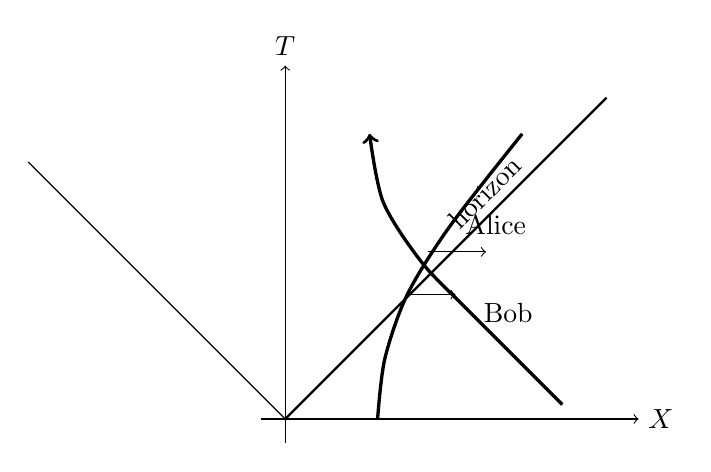
\begin{tikzpicture}[scale=1.02]
\draw[->] (-0.3,0) -- (4.4,0) node[right] {\(X\)};
\draw[->] (0,-0.3) -- (0,4.4) node[above] {\(T\)};
\draw[thick] (0,0) -- (4.0,4.0);
\draw[thin] (0,0) -- (-3.2,3.2);
\node[rotate=45,above] at (2.65,2.65) {horizon};
\draw[very thick]
  plot[smooth] coordinates {(1.15,0.0) (1.24,0.75) (1.52,1.55)
  (2.05,2.40) (2.95,3.55)};
\node[right] at (2.12,2.42) {Alice};
\draw[very thick,->]
  plot[smooth] coordinates {(3.45,0.18) (2.85,0.78) (2.25,1.38)
  (1.70,1.95) (1.22,2.70) (1.05,3.55)};
\node[right] at (2.35,1.32) {Bob};
\draw[->] (1.52,1.55) -- (2.12,1.55);
\draw[->] (1.78,2.08) -- (2.50,2.08);
\end{tikzpicture}
\caption{Alices beschleunigte Weltlinie im Außenbereich und Bobs Weltlinie im freien Fall. Alices Koordinatenschnitte nähern sich dem Horizont an; Bob überquert ihn in endlicher Eigenzeit.}
\end{figure}

\begin{classroomqa}
\audiencequestion{Was sieht Bob, wenn er zurück zu Alice blickt, und was geschieht nach dem Überqueren mit seiner Uhr?}
\lecturerresponse{Bob sieht, wie Alice sich mit der Beschleunigung entfernt, die nötig ist, um sie außerhalb zu halten; ein singuläres Ereignis beim Überqueren sieht er jedoch nicht. Alice kann bei festem Radius gehalten werden; eine Umlaufbahn wäre eine andere mögliche Anordnung. Bobs Uhr misst seine Eigenzeit \(\tau\) weiterhin ganz normal. Im Inneren beschreibt die Aussage, dass die Radialkoordinate zeitartig ist, die kausale Geometrie; sie verwandelt seine Armbanduhr nicht buchstäblich in einen Meterstab. Seine Weltlinie endet schließlich bei \(r=0\).
\lecturetimestamp{01:39:51--01:44:45}}
\end{classroomqa}

Nun erkennen wir die Nullgerade als den Horizont selbst, nicht bloß als einen Punkt, an dem sich ein Koordinatenkoeffizient auffällig verhält. Außerhalb bewegt sich eine Familie radialer Lichtstrahlen nach außen. Innerhalb führen beide zukunftsgerichteten Lichtkegelrichtungen zu kleineren Werten von \(r\). Jede zukunftsgerichtete Bahn eines massiven Teilchens muss zwischen diesen Nullrichtungen bleiben und erreicht daher die Singularität.

\section{Signale, Rotverschiebung und ein entstehender Horizont}

Nehmen wir an, kollabierende Materie sende eine regelmäßige Folge von Lichtpulsen aus. Ein weit entfernter Beobachter empfängt die späteren Pulse in immer größeren Zeitabständen. Ihre Frequenzen verschieben sich vom sichtbaren Licht über Infrarot, Mikrowellen und Radiowellen zu noch längeren Wellenlängen. In einer idealisierten klassischen Rechnung kann der Außenbeobachter weiterhin immer spätere Signale mit Materie in Verbindung bringen, die sich dem Horizont nähert; in der Praxis wird die Quelle jedoch rasch zu stark rotverschoben und zu lichtschwach, um noch nachweisbar zu sein.

\begin{classroomqa}
\audiencequestion{Sieht ein Außenbeobachter während des Kollapses einfach die gesamte Materie am Horizont einfrieren?}
\lecturerresponse{In Schwarzschild-Zeit nähert sich die Oberfläche der kollabierenden Materie asymptotisch dem Horizont und erscheint zunehmend eingefroren. Was tatsächlich beobachtet wird, zeigt sich in den Lichtsignalen, die immer stärker verzögert, rotverschoben und lichtschwächer werden. Diese Beschreibung in Koordinaten besagt nicht, dass die einfallende Materie unendlich viel Eigenzeit erlebt.
\lecturetimestamp{01:47:06--01:48:11}}
\end{classroomqa}

\begin{classroomqa}
\audiencequestion{Könnte ein hinreichend spät eintreffender Beobachter die gesamte Geschichte des Falls rekonstruieren?}
\lecturerresponse{Nur anhand von Signalen, die ausgesandt wurden und den Beobachter tatsächlich erreichen. Aufeinanderfolgende Pulse liegen zeitlich immer weiter auseinander und sind zunehmend rotverschoben. Ein idealer Beobachter mit unbegrenzter Empfindlichkeit könnte dem klassischen Signal bis zu immer längeren Wellenlängen folgen; ein Beobachter in der Praxis sieht das Objekt verblassen.
\lecturetimestamp{01:48:13--01:52:00}}
\end{classroomqa}

\begin{classroomqa}
\audiencequestion{Was bedeutet es genau, wenn man sagt, die Singularität sei eine Zeit und kein Ort?}
\lecturerresponse{Die Fläche \(r=0\) ist raumartig. Sobald man sich innerhalb des Horizonts befindet, endet jede zukunftsgerichtete zeitartige oder lichtartige Kurve dort. Einem räumlichen Ort kann man ausweichen, indem man einen anderen Weg wählt; einer zukünftigen Grenze kann man nicht ausweichen, solange man einer zukunftsgerichteten Weltlinie folgt.
\lecturetimestamp{01:52:02--01:53:10}}
\end{classroomqa}

Wie kann ein Schwarzes Loch dann entstehen oder an Masse zunehmen, wenn der Außenbeobachter nie sieht, wie Materie den Horizont überquert? Betrachten wir eine kollabierende Kugelschale. Der globale Horizont wartet nicht als vorab vorhandene materielle Fläche bei einem festen Radius. Er entsteht im Zentrum und wächst nach außen, bis er die kollabierende Schale erreicht und sich der Bereich des Schwarzen Lochs bildet. In der äußeren Schwarzschild-Beschreibung nähert sich die Schale weiterhin asymptotisch dem endgültigen Horizont. Das vollständige Raumzeitbild, einschließlich der globalen Bestimmung des Horizonts, ist Thema der nächsten Vorlesung.

\begin{figure}[htbp]
\centering
\includegraphics[width=0.90\textwidth]{lecture_06_figure_07.png}
\caption{Eine kollabierende Schale und der vom Zentrum nach außen wachsende Horizont, der auf sie trifft. Die Zeichnung gibt einen Ausblick auf die globale Kollapsgeometrie, die in der nächsten Vorlesung entwickelt wird.}
\lectureframe{01:57:25}
\end{figure}

\begin{classroomqa}
\audiencequestion{Wenn in der äußeren Koordinatenzeit nichts den Horizont überquert, wie kann dann ein Schwarzes Loch entstehen oder wachsen?}
\lecturerresponse{Die Voraussetzung vermischt eine Aussage über Koordinaten mit einer globalen Aussage. Die kollabierende Materie erreicht den maßgeblichen Bereich in endlicher Eigenzeit, während der Ereignishorizont durch die Kausalstruktur der gesamten Raumzeit bestimmt wird. Im Schalenbild entsteht er im Zentrum und wächst nach außen, bis er die Schale erreicht. Die verzögerte, rotverschobene Sicht des Außenbeobachters ist weiterhin mit diesem globalen Horizont vereinbar.
\lecturetimestamp{01:53:11--01:57:34}}
\end{classroomqa}

\section{Entweichungsrichtungen zwischen den beiden Sphären}

Der Horizont und die Photonensphäre unterteilen das Strahlungsproblem in verschiedene Fälle. Bei einem Radius
\begin{equation}
2MG<r<3MG,
\end{equation}
kann ein radial nach außen gerichteter Lichtstrahl bis ins Unendliche entkommen. Ein tangentialer Lichtstrahl kann das nicht; er fällt nach innen. Zwischen diesen Richtungen liegt ein Entweichungskegel. Je näher man dem Horizont kommt, desto enger wird dieser Kegel um die radiale Richtung nach außen. Nach dem Überqueren des Horizonts schließt er sich vollständig.

\begin{classroomqa}
\audiencequestion{Kann eine Lichtquelle zwischen Horizont und Photonensphäre ein Signal nach außen senden?}
\lecturerresponse{Ja. Ein hinreichend radial nach außen gerichteter Nullstrahl entkommt, solange sein Emissionsereignis außerhalb von \(2MG\) liegt. Die Aussage, dass Winkelbewegung innerhalb von \(3MG\) nach innen führt, schließt ein radiales Entkommen nicht aus. Entscheidend ist die Emissionsrichtung; der mögliche Entweichungskegel nach außen wird enger, je näher die Quelle dem Horizont kommt.
\lecturetimestamp{01:57:34--01:59:48}}
\end{classroomqa}

\begin{classroomqa}
\audiencequestion{Kann ein von außen kommender Strahl innerhalb der Photonensphäre vorbeiziehen, umkehren und wieder nach außen gelangen?}
\lecturerresponse{Nicht auf einer Nullgeodäte der hier betrachteten Art. An einem Umkehrpunkt wäre die radiale Geschwindigkeit null; der Strahl wäre dann bei einem Radius unterhalb von \(3MG\) momentan tangential. Dort führt die Winkelbewegung nach innen, statt den Strahl wieder nach außen zu lenken. Eine Quelle, die sich bereits zwischen den beiden Sphären befindet, kann dennoch einen hinreichend radial nach außen gerichteten Strahl aussenden, bevor sie den Horizont überquert.
\lecturetimestamp{01:59:49--02:01:27}}
\end{classroomqa}

Die letzte Frage ist absichtlich weniger eindeutig beantwortet. Man stelle sich vor, Alice und Bob würden beide auf demselben Radius außerhalb des Horizonts gehalten. Nahe beieinander befindliche Beobachter können offensichtlich Signale austauschen. Sind sie auf der Kugel weit voneinander entfernt, erfordern der direkte lichtartige Weg und seine begrenzte Winkelreichweite eine explizite Geodätenrechnung. Die Teilnehmer schlagen einen indirekten Weg vor: Die Nachricht wird nahezu radial nach außen zu einer Relaisstation in größerem Abstand vom Horizont gesandt, dort herumgeleitet und wieder nach innen gesandt. Eine andere Variante lässt einen nach außen geworfenen Gegenstand oder ein Signal umkehren und zurückkehren. Diese Wege zeigen, warum das Ausbleiben einer tangentialen Kreisbahn für sich genommen nicht jede Kommunikation zwischen Beobachtern außerhalb des Horizonts ausschließt.

\begin{classroomqa}
\audiencequestion{Können zwei Beobachter, die auf demselben Radius nahe am Horizont gehalten werden, rund um das Schwarze Loch miteinander kommunizieren?}
\lecturerresponse{Lokal gesehen: ja. Für weit voneinander entfernte oder diametral gegenüberliegende Beobachter wurde die Grenze für den direkten Weg in der Vorlesung nicht bestimmt; sie sollte daher nicht als Satz dargestellt werden. Zunächst bleibt die Frage nach den Winkelgeodäten offen. Dann wird festgestellt, dass ein indirektes Signal nahezu radial nach außen laufen, in größerem Radius herumgeleitet werden und zurückkehren kann. Je näher man dem Horizont kommt, desto schmaler wird der Winkelbereich, in dem ein direkter Weg nutzbar ist; außerhalb des Horizonts bleibt jedoch ein Weg nach außen möglich.
\lecturetimestamp{02:01:29--02:04:17}}
\end{classroomqa}

Im nächsten Schritt ersetzen wir diese Skizzen nahe am Horizont durch die globale Geometrie eines kollabierenden Körpers und untersuchen genau, wie ein Ereignishorizont wächst.